\documentclass[a4paper, 12pt]{article}%тип документа

%отступы
\usepackage[left=2cm,right=2cm,top=2cm,bottom=3cm,bindingoffset=0cm]{geometry}

%Русский язык
\usepackage[T2A]{fontenc} %кодировка
\usepackage[utf8]{inputenc} %кодировка исходного кода
\usepackage[english,russian]{babel} %локализация и переносы
\usepackage[unicode, pdftex]{hyperref}

%Вставка картинок
\usepackage{wrapfig}
\usepackage{graphicx}
\graphicspath{{pictures/}}
\DeclareGraphicsExtensions{.pdf,.png,.jpg}

%оглавление
\usepackage{titlesec}
\titlespacing{\chapter}{0pt}{-30pt}{12pt}
\titlespacing{\section}{\parindent}{5mm}{5mm}
\titlespacing{\subsection}{\parindent}{5mm}{5mm}
\usepackage{setspace}
\usepackage{caption}

%Графики
\usepackage{multirow}
\usepackage{pgfplots}
\pgfplotsset{compat=1.9}

%Математика
\usepackage{amsmath, amsfonts, amssymb, amsthm, mathtools}

%Стиль страницы
\usepackage{fancyhdr}
\pagestyle{fancy}

\begin{document}

\begin{titlepage}

\begin{center}
%\vspace*{1cm}
\large\textbf{Московский Физико-Технический Институт}\\
\large\textbf{(государственный университет)}
\vfill
\line(1,0){430}\\[1mm]
\huge\textbf{Проект по курсу <<Микроконтроллеры>>}\\
\huge\textbf{<<Калькулятор на LCD Keypad Shield>>}\\
\line(1,0){430}\\[1mm]
\vfill
\large Проект подготовили студенты 2 курса ФРКТ, группы Б01-007:\\
\large Сибгатуллин Булат\\
\large Шумаков Иван\\
\large Глухарева Дарья\\
\large Тимофеев Михаил\\
\end{center}

\end{titlepage}

\tableofcontents{} %содержание
\newpage

\section{Описание аппаратной платформы, на которой построен проект}

Данный проект создан на базе 8-битного микроконтроллера ATmega328P, построенного на архитектуре AVR с тактовой частотой 16 МГц. ATmega328P обладает 3-мя видами памяти:
\begin{itemize}
\item 32 КБ Flash-памяти, из которых 0,5 КБ используются загрузчиком, который позволяет прошивать Uno с обычного компьютера через USB. Flash-память постоянна и её предназначение — хранение программ и сопутствующих статичных ресурсов.

\item 2 КБ RAM-памяти, которые предназначены для хранения временных данных, например переменных программы. По сути, это оперативная память платформы. RAM-память энергозависимая, при выключении питания все данные сотрутся.

\item 1 КБ энергонезависимой EEPROM-памяти для долговременного хранения данных, которые не стираются при выключении контроллера. По своему назначению это аналог жёсткого диска для Uno.
\end{itemize}

Данный микроконтроллер установлен на аппаратную платформу Arduino UNO. Микроконтроллер ATmega328P не содержит USB интерфейса, поэтому для прошивки и коммуникации с ПК на плате присутствует дополнительный микроконтроллер ATmega16U2 с прошивкой USB-UART преобразователя. При подключении к ПК Arduino Uno определяется как виртуальный COM-порт.

Сама аппаратная платформа Arduino UNO обладает:
\begin{enumerate}
\item 3-мя светодиодами:

\begin{itemize}
\item Индикатор питания платформы.

\item Пользовательский светодиод на 13 пине микроконтроллера.

\item RX и TX индикатор отображующий статус прошивки микрокотроллера.
\end{itemize}

\item Портом USB Type-B, предназначенный для прошивки и питания платформы.

\item Разъём питания DC, придназначенный для подключения внешнего источника напряжения от 7 до 12 вольт.

\item Понижающий регулятор 5V, обеспечивающий питание микроконтроллера и другой логики платы при подключении питания через разъём питания DC или пин Vin. Диапазон входного напряжения от 7 до 12 вольт. Выходное напряжение 5 В с максимальным выходным током 1 А.

\itemПонижающий регулятор 3V3, обеспечивающий напряжение на пине 3V3. Регулятор принимает входное напряжение от линии 5 вольт и выдаёт напряжение 3,3 В с максимальным выходным током 150 мА.

\item Кнопка сброса, предназначеная для ручного сброса прошивки — аналог кнопки RESET обычного компьютера.

\item Два ICSP разъёма, по одному на каждый микроконтроллер на платформее.
\end{enumerate}

Распиновка аппаратной платформы Arduino UNO представлена на рис. 1.

\newpage

%Вставка изображения
\begin{figure}[h!]
\centering
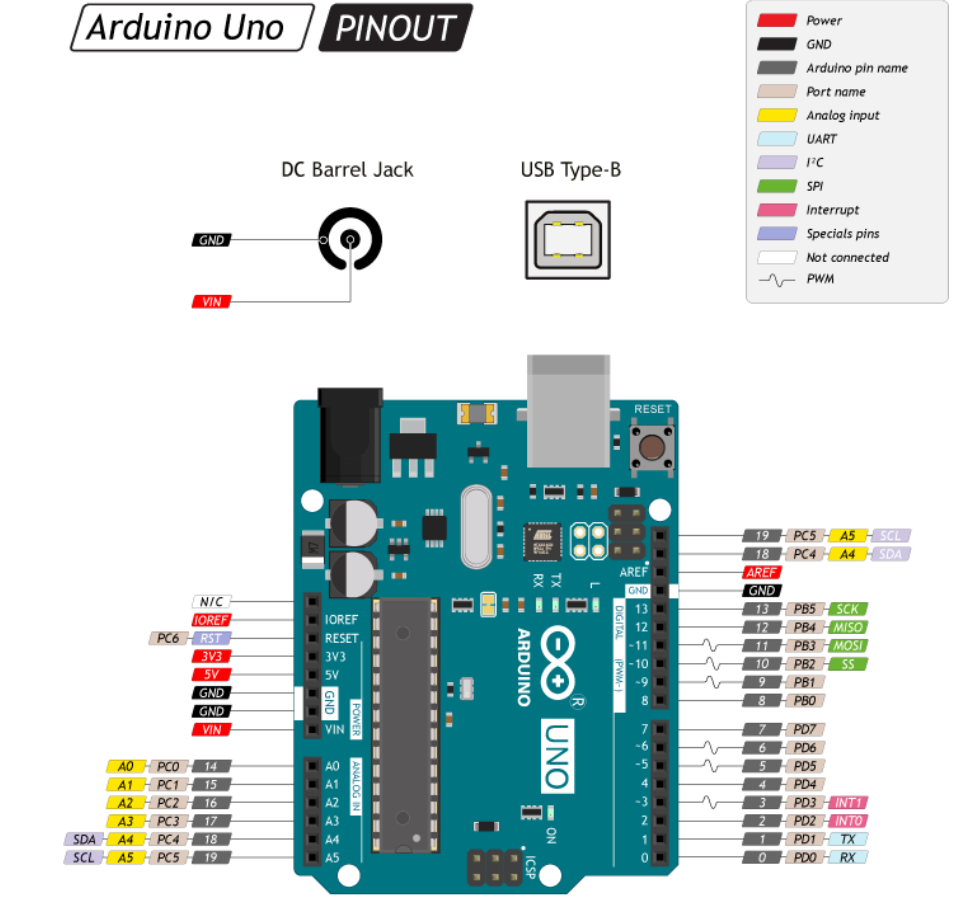
\includegraphics[scale=0.6]{images/Arduino_UNO-pinout.png}
\caption{Распиновка Arduino UNO}
\label{Arduino_UNO-pinout}
\end{figure}

На рис. 2 можно наблюдать монтажную схему используемой платформы.

\begin{figure}[h!]
\centering
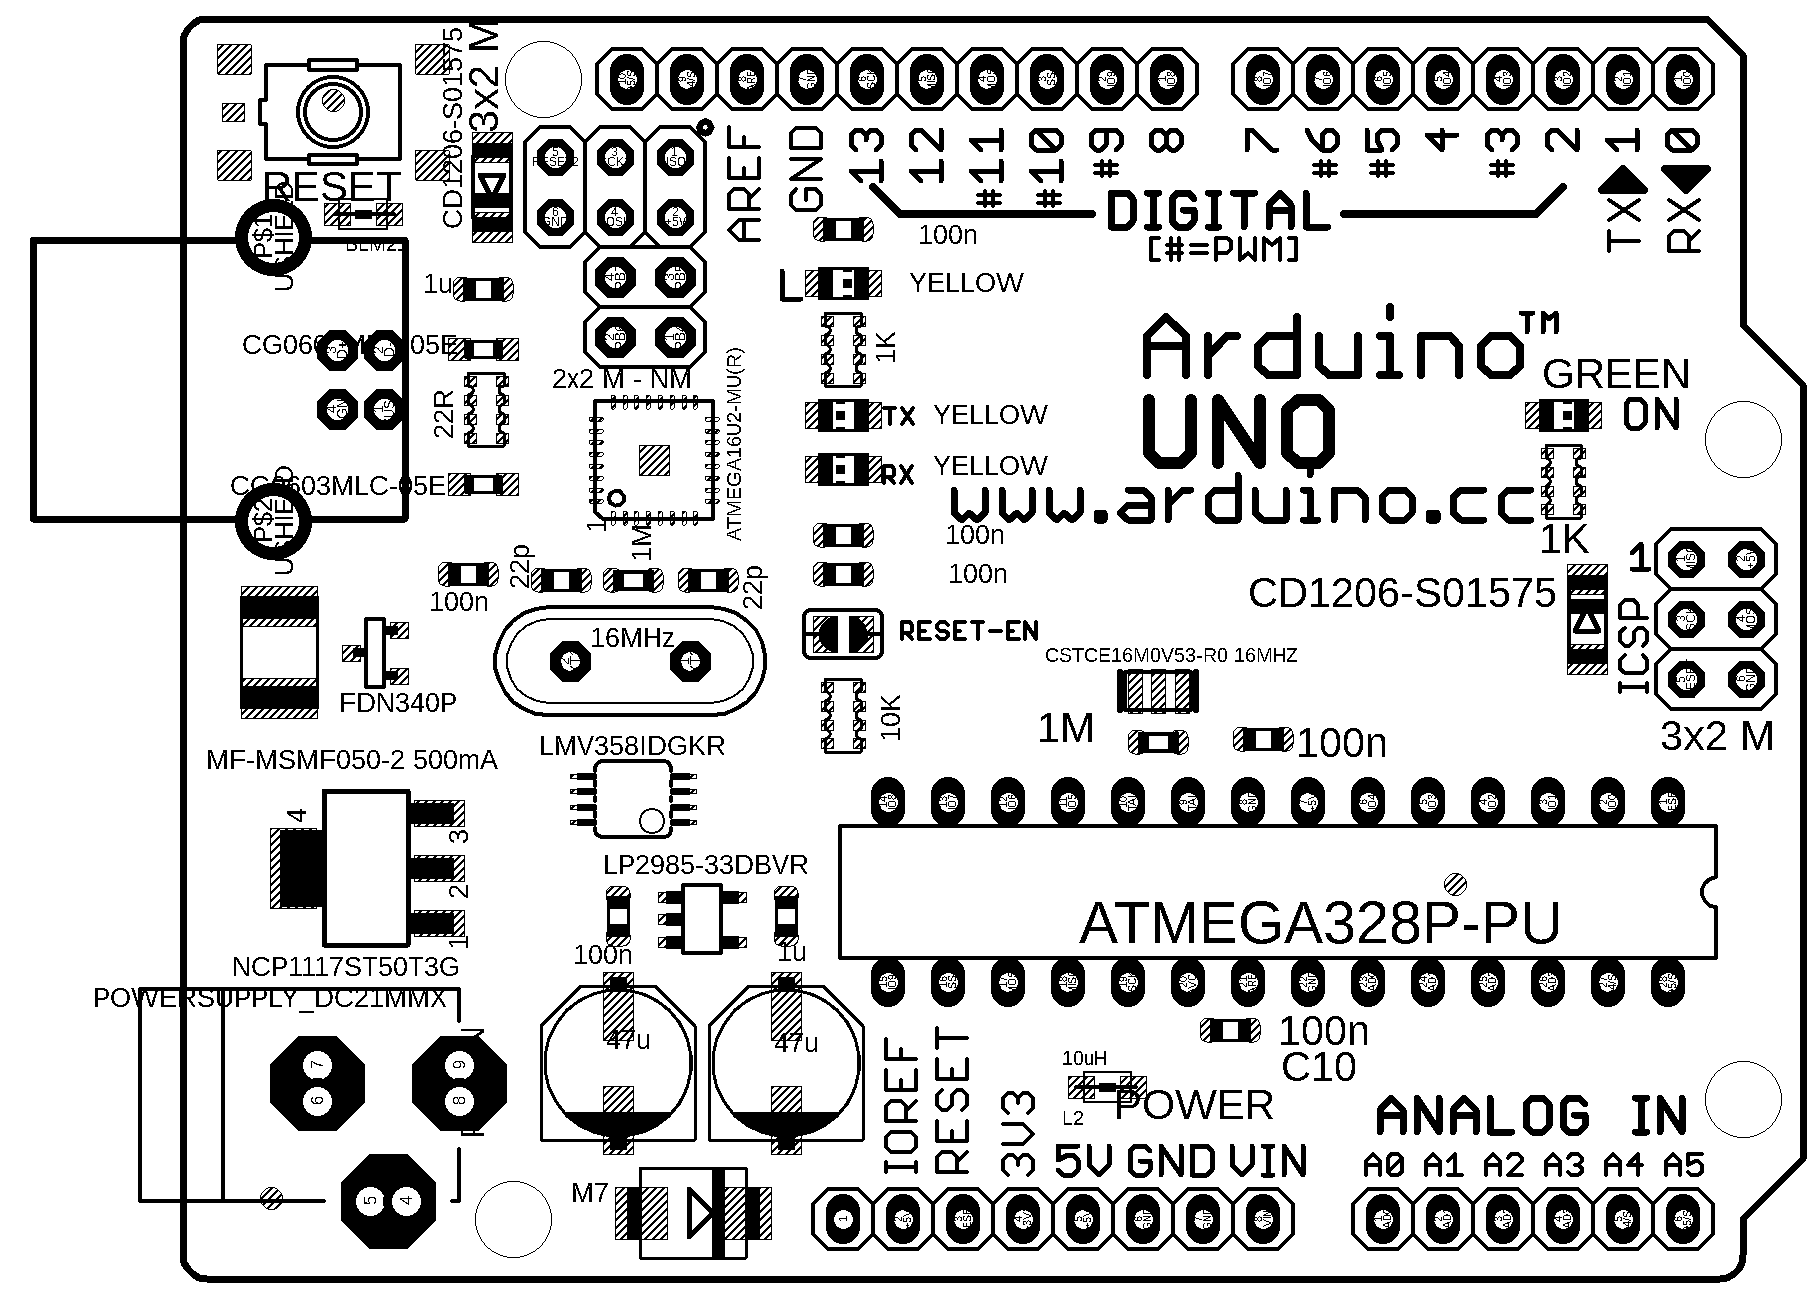
\includegraphics[scale=0.2]{images/arduino-uno-layout-top.png}
\caption{Монтажная схема Arduino UNO}
\label{arduino-uno-layout-top}
\end{figure}

\newpage

\section{Описание модуля LCD Keypad Shield}

Для работы с Arduino UNO используется модуль LCD Keypad Shield. Рассматриваемый шилд представляет собой плату с встроенными модулями индикации и управления. Индикация осуществляется с помощью LCD-дисплея TC1602, управление – через встроенные кнопки. Есть возможность регулировки яркости дисплея прямо на плате с помощью подстроечного резистора. Плата снабжена разъемами, в которые могут быть подключены другие устройства, например, датчики.

Небольшая информация о технических характеристиках устройсва:

\begin{itemize}
\item Тип дисплея: LCD 1602, символьный, 4-х битный режим.

\item Разрешение: 16×2 (две строки по 16 символов каждая). Знакоместо 5×8 точек.

\item Цвет дисплея: синий. Буквы белого цвета.

\item Технология: STN, Transflective, Positive.

\item Контроллер дисплея: HD44780U.

\item Предельная частота обновления экрана: 5Гц

\item Питание дисплея: 5 Вольт

\item Кнопки: 6 кнопок (5 кнопок управления и Reset).

\item Дополнительные элементы: регулировка яркости подсветки (потенциометр).
\end{itemize}

Также на шилде расположен светодиод, отображающий информацию о питании платы, и котактные площадки для подключения аналоговых устройств.

Для подлкючения шилда к Ардуино при помощи монтажной платы можно использовать распиновку, представленную на рис. 3.

В нашем случае подключение производится обычным <<насаживанием>> шилда на плату, нужно просто попасть ножками в соответствующие разъёмы платы Arduino и аккуратно совместить их.

Для работы с экраном используется библиотека LiquidCrystal (которая подходит для большинства LCD экранов).

\newpage

\begin{figure}[h!]
\centering
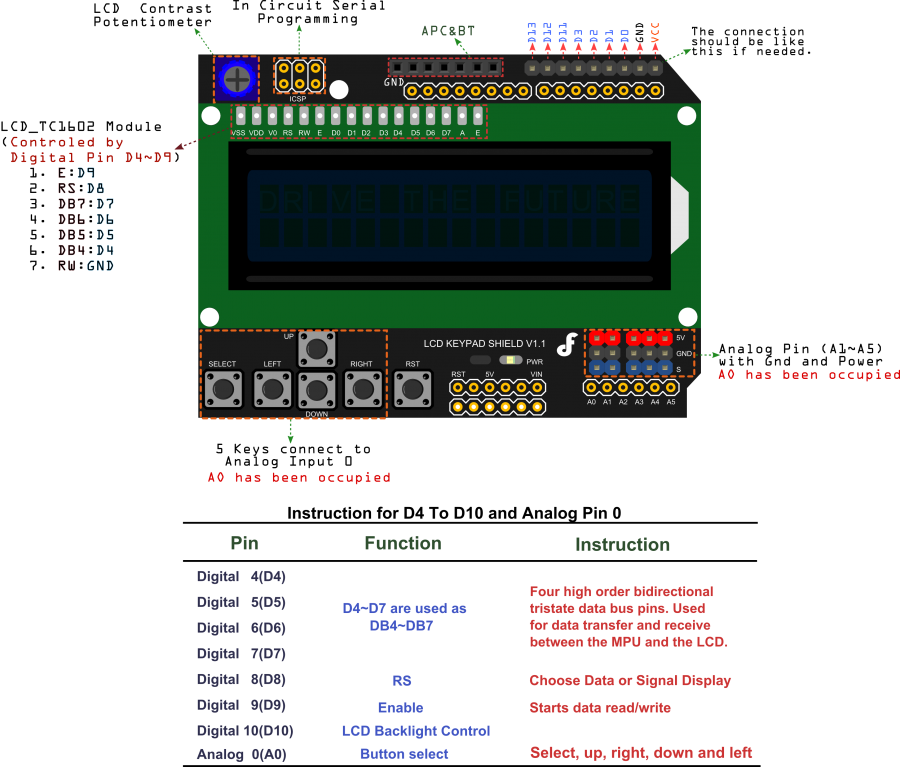
\includegraphics[scale=0.4]{images/900px-DFR0009-PIN2.png}
\caption{Распиновка модуля LCD Keypad Shield}
\label{900px-DFR0009-PIN2}
\end{figure}

\newpage

\section{Описание проекта и код}

Код написан на языке C++ и состоит из двух файлов Calculator.ino и main.ino (*.ino это стандартное расширение используемое для работы с аппаратной платформой Arduino):

\begin{itemize}
\item Файл Calculator.ino содержит в себе информацию о классе Calc, способную распознавать в строках математические выражения и в случае, если выражение правильно записано, возвращать его результат.

\item Файл main.ino содержит в себе методы работы с LCD экраном, такие как вывод на него информации, управление экраном при помощи кнопок и считывание информации записанной на экране.
\end{itemize}

Для работы с данным калькулятором пользователю предлагается ввести в верхнюю строку математическое выражение. Выбирать символ можно при помощи кнопок UP и DOWN, расположенных на шилде. Перемещать курсов можно при помощи кнопок RIGHT и LEFT. После того, как выражение записано и пользователь хочет вычислить его результат, он должен нажать кнопку SELECT. В случае если выражение математически верно, в нижней строке будет записан результат вычислений, в обратном же случае в нижней строке будет выведено: <<syntax error>>.

Сам код проекта можно посмотреть по ссылке: \url{https://github.com/Zararest/Arduino_calculator}. Код находится в папке Calculator, в уже упоминавшихся файлах Calculator.ino и main.ino. Загрузку кода на микроконтроллер ATmega328P можно осуществить при помощи среды разработки Arduino IDE, предварительно подключив платформу Arduino UNO к одному из портов компьютера.
\end{document}